\documentclass[11pt]{article}
\usepackage[margin=0.85in]{geometry}
\usepackage{amsmath,amssymb,graphicx,hyperref}
\hypersetup{breaklinks=true}
\setlength{\parindent}{0pt}
\setlength{\parskip}{7pt}
\begin{document}
{\Large Exact polynomial norm and matrix witness equivalence}\\
November 13, 2026. Unsigned producer evidence [pcc:unverified].

\textbf{Construction.} For a field $K$, finite index set $I$, supplied polynomial
families $A_i,B_i\in K[X]$, and $f\in K[X]$, put
\[
 A_w=\sum_i w_i A_i,\quad B_w=\sum_i w_i B_i,\quad
 L(M)=\sum_{i,j} M_{ij}(A_iA_j-f B_iB_j).
\]
For target coordinates $q,y\in K$, set $\ell_i=A_i(q)-yB_i(q)$.
Lean checks the actual polynomial identities
\[
 L(ww^T)=A_w^2-fB_w^2,\qquad
 \sum_i w_i\ell_i=A_w(q)-yB_w(q).
\]

\textbf{Exact witness theorem.} If $G\in K[X]$ is nonzero, then the existence
of $w$ and $c\ne0$ with
\[
 A_w^2-f B_w^2=cG,\qquad A_w(q)-yB_w(q)=0
\]
is equivalent to the existence of a nonzero symmetric matrix $M$ and $c\ne0$
with all two-by-two minors zero, $M\ell=0$, and $L(M)=cG$.
The coefficient vector $w$ is not assumed nonzero: the nonzero norm equation
proves that condition. The theorem concerns the spans of the supplied families.

\begin{center}
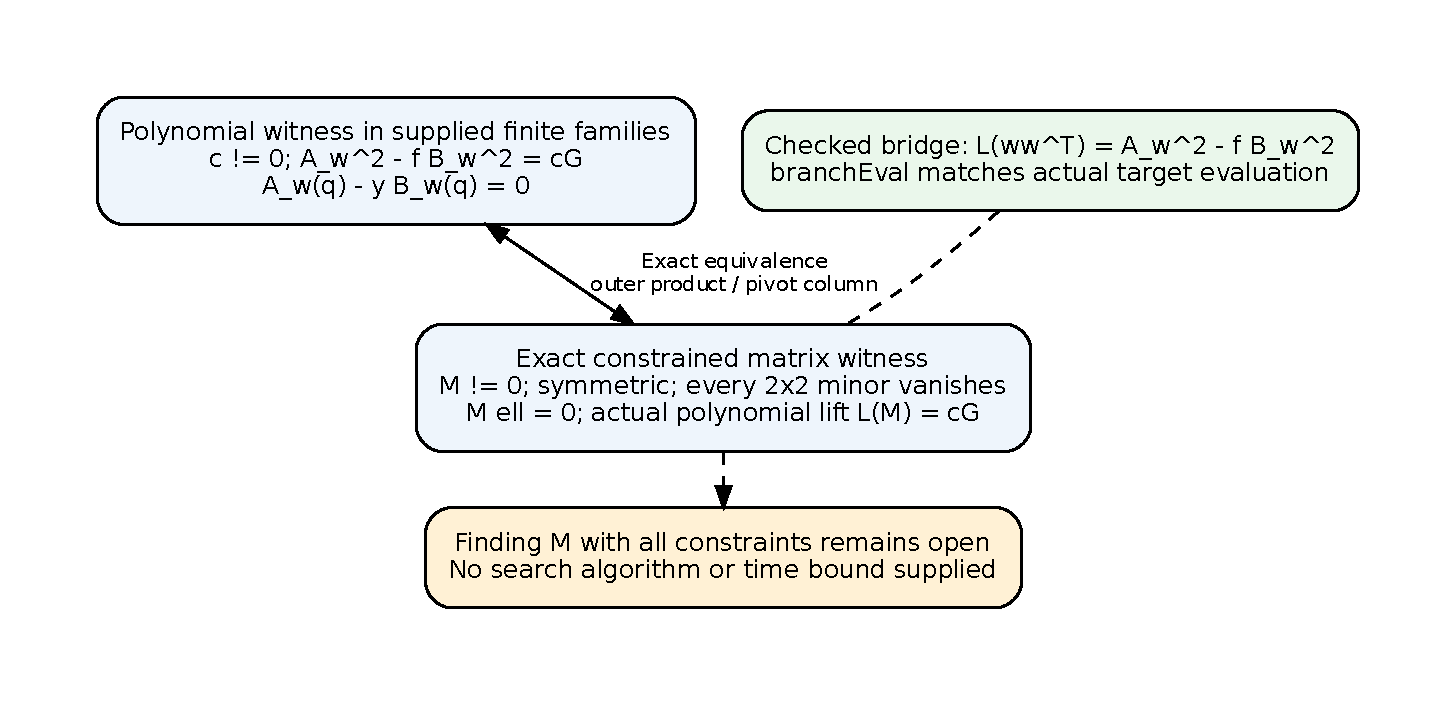
\includegraphics[width=0.92\linewidth,height=0.37\textheight,keepaspectratio]{equivalence.pdf}
\end{center}

\newpage
{\Large Proof, formal scope and evidence}

\textbf{Forward direction.} Use $M=ww^T$. Nonzero $cG$ excludes $w=0$,
so one diagonal entry $w_k^2$ is nonzero. Symmetry and every minor equation
follow from the outer product. The branch identity gives $M\ell=0$;
the norm expansion gives the actual polynomial lift equation.

\textbf{Reverse direction.} For a nonzero symmetric minor-vanishing matrix,
a nonzero diagonal pivot $M_{kk}$ exists. Set $w_i=M_{ik}$ and
$s=M_{kk}^{-1}$. Then $M=sww^T$, $s\ne0$. Its pivot row and symmetry give
$\sum_i w_i\ell_i=0$. Linearity of the defined lift gives
$A_w^2-fB_w^2=(c/s)G$, with $c/s\ne0$. No square root or extension field
is needed. The reverse implication itself does not require $G\ne0$.

\textbf{Proof map.} Module \path{NormLift}: \path{outerNorm},
\path{branchEval}, \path{witnessVectorNonzero}, \path{normToMatrix},
\path{matrixToNorm}, \path{witnessEquivalence}. The extraction module
additionally supplies \path{outerMinors}; its earlier
five claimed theorem declaration hashes are unchanged. Explicit minor equations
are used, without assuming a numerical-rank oracle.

\textbf{Evidence.} Source commit \path{9cba2446b}; Lean 4.35.0 and pinned
manifest. Default build004 passed3143 jobs. Actual tracked-source audit:
28 declarations, zero additional trusted axioms. Printed foundations are
\path{propext}, \path{Classical.choice}, \path{Quot.sound} only.
Fresh import-inclusive status is recorded in the norm-lift evidence directory's
\path{fresh-status.json}.
Builds002/003 failed at an imported definition's module interface and are retained
as failures. The public minor constructor resolves that boundary.

Native record \path{IDC1h2e7ff8ae9d53fc24} supplements the four-component
expansion with32 statement-derived and32 extra checker-stream points and a source
hash. It does not execute Lean or certify arbitrary arity by sampling. The Lean
proof provides the universal finite-index identity. New PCC claim bindings are
unsigned and retained in \path{norm-lift-evidence/claim-pins.json}.

\textbf{Remaining dependencies.} Monomial-basis degree completeness, the complete
curve/divisor/group bridge, and an algorithm for finding the constrained matrix
are separate. No search-time bound is established. No experiment, performance
measurement, target solve or universal lower bound is reported.

\textbf{Sources.} Pinned Mathlib polynomial evaluation and linear-map lemmas;
Galbraith's norm/divisor sections linked in \path{sources.json}; the Nov13
non-Semaev note as scoped context. KB unavailable; no novelty is claimed for
this elementary lifting construction. Existing historical graphs remain unchanged.
\end{document}
